%% Template for MLP Coursework 4

%% Based on  LaTeX template for ICML 2017 - example_paper.tex at 
%%  https://2017.icml.cc/Conferences/2017/StyleAuthorInstructions

\documentclass{article}
\input{mlp2021_includes}

%% You probably do not need to change anything above this comment

%% REPLACE this with your project title, group ID and list of student numbers for the group
\def\projectTitle{Optimization of CycleGAN Model}
\def\groupNumber{G071}
\def\studentNumbers{s2056595, s2123157, s2196789}

\begin{document} 

\twocolumn[
\mlptitle{\projectTitle: Final Report}

\centerline{\groupNumber\ (\studentNumbers)}

\vskip 7mm
]

\begin{abstract} 
The purpose of image-to-image translation is to learn the mapping between an input picture and an output image using a training set of matched image pairings. When matched training data is unavailable, CycleGAN provides a method for learning how an image may be translated from one source domain to another. While CycleGAN's strategy often produces persuasive findings, the outcomes are far from universally good. Certain types of failures are triggered by the distribution properties of the training datasets. Additionally, we notice a persistent discrepancy between the outcomes obtained using paired training data and those from unpaired strategy. Managing increasingly complex and intense transformations, particularly geometrical transformations, is the main purpose of our evaluation of a new modified unsupervised generative model with attention. Unpaired data is not necessary for unsupervised generative networks, which is reflected in the CycleGAN structure. Weights in the feature map indicate attention, which can partition the source domain from the target domain using the auxiliary classifier's attention map. We present an adaptive hybrid normalisation layer composed of LN and IN to assist attention-guided models in controlling the amount of shape and texture variation without adjusting the model architecture or hyper-parameters.
\end{abstract} 

\section{Introduction}
\label{sec:intro}
While the image to image translation problems has been widely investigated since the first generation of Generative Adversarial Networks(GAN) was invented in June, 2014 by Ian Goodfellow et al, the most state-of-art method for this field of tasks is still being pursued by people year by year\cite{GAN}. Image-to-image translation has a wide range of applications including changing a carton photo to a realistic photo, or converting real landscape map to satellite map. However, at the early stage of the work, people were required to collect large amount of paired dataset for training neural networks, which is called pix2pix\cite{Conditional}. In reality, it is usually very difficult to collect paired images due to the constraints of different situations, and hence the generated results are not quite satisfactory. Purposed by Jun-Yan Zhu et al, in 2017, CycleGAN had greatly improve the performance in tasks of image-to-image translation, and became very popular as a state-of-art method\cite{cycle}.

The most significant improvement in CycleGAN is that it doesn't require paired images, which means we only need to care about one kind of images if we want to translate from A to B.The architecture of CycleGAN consists of two Generative models and two discriminator models. The function of generator $G$ maps from $X$ to $Y$ such that the distribution of $X$ are reproduced in the generated results $G(X)$, and the generator $F$ works exactly in the opposite direction. 

There are some limitations about CycleGAN. Although it has good performance on tasks involving texture or color transformation, such as converting horses to zebras, it does not perform well on geometrical translations. In some examples of geometrical translations it fails to translate from cat to dog. Some distributions of features would also lead to failure, as CycleGAN is incapable of learning multimaps from unpaired data \cite{Augmented_cyclegan}. For instance, when translating from horses to zebras, it doesn't consider there could be a man on the horses and as a result the man was also covered with zebra stripes\cite{intro}.

In this report we aim to assess a new modified unsupervised generative model with attention. We will test, verify, and evaluate the enhanced metrics and optimization effects in comparison to CycleGAN based on the model's principle of Generative Adversarial Networks.

This study's findings and indicators are excellent. The following are the primary features of this modified model with attention that are worth noting:

$\bullet$ Unsupervised Generative Networks: Reflected in the CycleGAN structure, unpaired data is not required.

$\bullet$ Attention \cite{Attention}: It is reflected in the feature map with weight. The specific tactic is to assist the model in determining where to focus the transformation by separating the source domain from the target domain through using attention map obtained by auxiliary classifier.

$\bullet$ Adaptive Normalization Layer: An adaptive hybrid normalization layer of LN and IN is introduced to help our attention-guided model flexibly control the amount of shape and texture variation without modifying the model architecture or hyper-parameters.

\section{Data set and task} 
In this report, we use multiple datasets to accomplish different image-to-image translation tasks based on our modified model. We use the same data as used in CycleGAN \cite{EECSB} \textbf{horse2zebra}, \textbf{apple2orange},  \textbf{summer2winter}, and \textbf{iphone2dslr\_flower} . Additionally, we introduce extrinsic dataset like \textbf{cat2dog} \cite{CvsD}. We also use \textbf{selfie2anime} for testing the style transfer. For data set in each task, we separate training set and test set for two domains in our task. For each domain, we choose around 1000 images as training set and around 100 images as test set. 


We aim to explore three representative image-to-image translation tasks which separately focusing on geometric changes, texture and color changes, and style changes. For each task, We specifically choose appropriate datasets to achieve it goals. 

In task of geometric changes, we use \textbf{cat2dog} and \textbf{apple2orange} dataset to convert cats to dogs and convert apple to orange. \textbf{cat2dog} and \textbf{apple2orange} are datasets used to evaluate CycleGAN's proposed future optimization direction, which may successfully assess the function of attention in the conversion process via our modified model. 

In task of texture and color changes, for \textbf{horse2zebra} dataset,we convert horses to zebra by changing textures and color of horses in the photo. For \textbf{summer2winter} and \textbf{iphone2dslr\_flower} dataset to change.

In task of style changes, we use \textbf{selfie2anime} to convert photo styles from selfie to anime. The anime set includes several figures of anime characters with different drawing styles.


\section{Methodology}

\subsection{CycleGAN}
Our objective is to discover mapping functions between two domains $\textit{X}$ and $\textit{Y}$ using training data  $\{x_i\}^{N}_{i=1}$ where $x_i \in X$ and $\{y_i\}^{N}_{j=1}$ where $y_i \in Y$. The data distribution is denoted by the variables $x \sim p_{data}(x)$ and $y \sim p_{data}(y)$. Our model, as indicated, has two mappings: $G: X \rightarrow Y$ and $F: Y \rightarrow X$. Additionally, we present two adversarial discriminators $D_X$ and $D_Y$, where $D_X$ seeks to differentiate between pictures $\{x\}$ and translated images $\{F(y)\}$ and $D_Y$ seeks to distinguish between images $\{y\}$ and $\{G(x)\}$. Our aim includes two kinds of terms: \textit{adversarial losses} for matching the distribution of produced pictures to the distribution of data in the target domain; and \textit{cycle consistency losses} for preventing the learned mappings $\textit{G}$ and $\textit{F}$ from contradicting one another.
\subsubsection{Adversarial Loss}
Both mapping functions are susceptible to adversarial losses\cite{AL}. The aim for the mapping function $G: X \rightarrow Y$ and its discriminator $D_Y$ is as follows:
$$\mathcal{L}_{GAN}(G, D_X, Y, X) = \mathbb{E}_{y \sim p_{data}(y)}[logD_Y(y)] $$$$+ \mathbb{E}_{x \sim p_{data}(x)}[log(1 - D_Y(G(x)))]$$
in which $G$ attempts to produce pictures $G(x)$ that resemble images from domain $Y$, and $D_Y$ attempts to differentiate between translated samples $G(x)$ and genuine samples $y$. $G$ seeks to reduce this goal whereas $D$ seeks to enhance it, i.e., $min_G$ $max_{D_Y}$ $\mathcal{L}_{GAN} (G, D_Y, X, Y)$. We also include an adversarial loss for the mapping function $F: Y \rightarrow X$ and its discriminator $D_X$: $min_F$ $max_{D_X}$ $\mathcal{L}_{GAN}(F, D_X, Y, X)$.
\subsubsection{Cycle Consistency Loss}
It is theoretically possible to learn mappings $G$ and $F$ that yield identically distributed outputs as target domain $Y$ and $X$, respectively, using adversarial training (strictly speaking, this requires $G$ and $F$ to be stochastic functions)\cite{Strictly}. Any random permutation of pictures in the target domain, in contrast, may induce an output distribution that matches the target distribution when a network's capacity is high enough. A learnt function's ability to map an individual input $x_i$ to a desired output $y_i$ cannot be guaranteed by adversarial losses alone. We suggest that the learnt mapping functions should be cycle-consistent in order to further minimise the number of viable mapping functions. We use a loss in cycle consistency as a reward for this conduct:
$$\mathcal{L}_{cyc}(G, F) = \mathbb{E}_{x \sim p_{data}(x)}[\Vert{F(G(x)) - x\Vert}_1] $$$$+ \mathbb{E}_{y \sim p_{data}(y)}[\Vert{G(F(y)) - y\Vert}_1]$$
Reconstructed pictures $F(G(x))$ end up matching closely to the input images $x$ because of cycle consistency loss.
\subsubsection{Full Objective}
Ultimately, our goal is to accomplish the following:
$$\mathcal{L}(G, F, D_X, D_Y) = \mathcal{L}_{GAN}(G, D_Y, X, Y)$$
$$+ \mathcal{L}_{GAN}(F, D_X, Y, X) +\lambda\mathcal{L}_{cyc}(G, F)$$
In this case, $\lambda$ is used to regulate the relative relevance of the two goals. We're here to address:
$$G^*, F^* = arg \ min(G, F) \ max(D_X, D_Y) \ \mathcal{L}(G, F, D_X, D_Y)$$
Not that our model may be considered as training two "autoencoders"\cite{Autoencoders}: we learn one $F \circ G: X \rightarrow X$ and another $G \circ F: Y \rightarrow Y$ concurrently. Each of these autoencoders, however, has a unique internal structure: they map a picture to itself through an intermediate representation, which is a translation of the image into another domain. This configuration may alternatively be thought of as a subset of "adversarial autoencoders"\cite{AA}, which use an adversarial loss to train an autoencoder's bottleneck layer to match an arbitrary target distribution. In our scenario, the $X \rightarrow X$ autoencoder's target distribution is the domain $Y$.

\subsection{Modified Unsupervised Generative Model with Attention}

\subsubsection{Generator}
First, the image goes through a down-sampling module, and then through residual blocks to obtain the encoder feature map, which is divided into two paths. One is to obtain the weight information of each feature map through an auxiliary classifier, and then multiply it with the encoder feature map of the other path to obtain the attention feature map. The attention feature map is still divided into two paths. One goes through a 1x1 convolution and activation function layer to get the $a_1...a_n$ feature map, and then the feature map passes through the fully connected layer to get the $\gamma$ and $\beta$ of the Adaptive Layer-Instance Normalization layer in the decoder. The other path serves as the decoder's input, and the generated result is obtained through adaptive residual blocks (including Adaptive Normalization Layer) and an up-sampling module.

\begin{figure}
\centerline{\includegraphics[width=1\columnwidth]{Images/Generator.png}}\caption{The structure of the \textbf{Generator}}
\label{fig:Generator}
\end{figure} 

\subsubsection{Adaptive Normalization Layer}
Informed by recent research that employs affine transformation parameters in normalisation layers and the combination of normalisation functions \cite{Arbitrary}\cite{Batch-Instance}, the precise formula we provide is as follows:
$$ \hat{a}_{I}=\frac{a-\mu_{I}}{\sqrt{\sigma_{I}^{2}+\epsilon}}, \hat{a}_{L}=\frac{a-\mu_{L}}{\sqrt{\sigma_{L}^{2}+\epsilon}} $$
The above is the normalisation formula for IN and LN, after which $\hat{a}_{I}$ and $\hat{a}_{L}$ are substituted for merging ($\gamma$ and $\beta$ are passed in externally):
$$ \operatorname{AdaLIN}(a, \gamma, \beta)=\gamma \cdot\left(\rho \cdot \hat{a}_{I}+(1-\rho) \cdot \hat{a}_{L}\right)+\beta $$
To avoid $\rho$ from exceeding the range of $[0,1]$, the interval of $\rho$ is trimmed as follows:
$$ \rho \leftarrow c l i p[0,1](\rho-\tau \Delta \rho) $$
While AdaIN is capable of transferring content features to style features, AdaIN relies on the assumption that feature channels are uncorrelated \cite{Arbitrary}, which indicates that style features should include a huge number of content patterns, whereas LN does not \cite{Layer_normalization}. However, because LN considers global statistics, it would be unable to maintain the content structure of the original domain. As a result, we integrate AdaIN and LN and leverage their combined capabilities to selectively preserve or update content information, therefore assisting in the resolution of a broad variety of image-to-image translation difficulties.

\subsubsection{Discriminator}
The discriminator is significantly simpler than the generator whose particular structure is similar to the generator, but it employs spectral normalisation to improve training stability and convergence, and it uses leakyrelu for the activation function.

\begin{figure}
\centerline{\includegraphics[width=1\columnwidth]{Images/Discriminator.png}}\caption{The structure of the \textbf{Discriminator}}
\label{fig:Discriminator}
\end{figure} 

\subsubsection{Adversarial Loss}
The adversarial loss function is not the original log function \cite{Least}, but rather the MSE function.
$$ \begin{aligned} L_{GAN}^{s \rightarrow t} &=\left(\mathbb{E}_{x \sim X_{t}}\left[\left(D_{t}(x)\right)^{2}\right]+E_{x \sim X_{s}}\left[\left(1-D_{t}\left(G_{s \rightarrow t}(x)\right)\right)^{2}\right]\right) \end{aligned} $$ 
\subsubsection{Cycle Loss}
Under the CycleGAN architecture, the cycle consistency loss is as follows: A is translated to B, and then B is translated to A'; A and A' must be identical, and the loss is L1loss.
$$ L_{Cycle}^{s \rightarrow t}=\mathbb{E}_{x \sim X_{s}}\left[\left|x-G_{t \rightarrow s}\left(G_{s \rightarrow t}(x)\right)\right|_{1}\right] $$
\subsubsection{Identity Loss}
Identity loss assures that the colour distributions of the input and output images are similar.
$$ L_{Identity}^{s \rightarrow t}=\mathbb{E}_{x \sim X_{t}}\left[\left|x-G_{s \rightarrow t}(x)\right|_{1}\right] $$
\subsubsection{Class Activation Map (CAM) Loss}

The purpose of CAM \cite{U-GAT-IT} is to utilise the information from the auxiliary classifiers $\eta_{s}$ and $\eta_{D_{t}}$ to determine where they need to be improved, or what the largest disparity between the two domains is in their current state, which $G_{s \rightarrow t}$ and $D_{t}$ find out, given an image $x \in\left({X_{s}, X_{t}}\right)$.

The generator's CAM loss, calculated using BCE loss:
$$ \begin{aligned} L_{\text {CAM}}^{s \rightarrow t} &=-\mathbb{E}_{x \sim X_{s}}\left[\log \left(\eta_{s}(x)\right)\right]+\mathbb{E}_{x \sim X_{t}}\left[\log \left(1-\eta_{s}(x)\right)\right] \end{aligned} $$
The discriminator model had a significant error in the formulation provided by the original paper we referenced, which we addressed and corrected. The discriminator's CAM loss as measured by MSE:
$$ \begin{aligned} L_{c a m}^{D_{t}} &=\mathbb{E}_{x \sim X_{t}}\left[\left(\eta_{D_{t}}(x)\right)^{2}\right]+\mathbb{E}_{x \sim X_{s}}\left[\left(1-\eta_{D_{t}}\left(G_{s \rightarrow t}(x)\right)\right)^{2}\right] \end{aligned} $$




\section{Experiments}
\label{sec:expts}
\subsection{Overview}
In this experiment we trained the models on two frameworks, the one with typical CycleGAN architecture and the one with some modification which is built upon the architecture of CycleGAN. In order to evaluate the performance of both frameworks, we ran experiments on both framework on the same dataset for comparison. Different dataset will be used for testing different scenarios. The dataset we used in this experiment are \textbf{horse2zebra}, \textbf{apple2orange}, \textbf{cat2dog}, \textbf{summer2winter}, \textbf{iphone2dslr\_flower} and \textbf{selfie2anime}. 

For the sake of controlling variables, we keep the hyperparameters the same for all dataset we used. The crop size was capped at 256 for each image in order to assure that the desire target is included in the image. In the training process we use minibatch with size of 10 at each iteration. We also tried to decrease the size of each image to increase the training speed, but the loss of generators was fluctuated and did not converge, so we choose 256 by 256 as the input dimension of our model. We use adaptive learning rate with initial value of 0.0001. The total number of trianable parameters are showed in table\ref{tab:parameters}. 


\begin{figure*}[tb]
\begin{center}
\centerline{\includegraphics[width=2\columnwidth]{Images/loss.pdf}}
\caption{CAM loss, Identity loss, Cycle loss, Generator loss, and Discriminator loss of A, on \textbf{cat2dog} dataset}
\label{fig:loss}
\end{center}
\end{figure*} 

\begin{table}[tb]
\vskip 3mm
\begin{center}
\begin{small}
\begin{sc}
\begin{tabular}{lcccr}
\hline
Model name & G\_A(M) & G\_B(M) & D\_A(M) & D\_B(M) \\
\hline
CycleGAN    & 11.378 & 11.378 & 2.765 & 2.765 \\
Modified Model & 10.59 & 10.59 & 53.13 & 53.13\\
\hline
\end{tabular}
\end{sc}
\caption{Number of trianable parameters of CycleGAN and our modified model.}
\label{tab:parameters}
\end{small}
\end{center}
\vskip -3mm
\end{table}

\subsection{Model Modification}

There are some notable modifications that are made on typical CycleGAN architecture. Table\ref{tab:parameters} shows that the number of parameters of discriminator in modified model is far greater than that of parameters of discriminator in CycleGAN. This is because we add two extra discriminators for multi-scale model, one for global and the other one for local. The discriminator for global has receptive field of 190 and 7 convolutional layers, and that for local has receptive field of 46 and 5 convolutional layers. The active layer after each convolutional layer is leaky ReLU. The reason why we use this multi-scale model is that we want to discriminate pictures in different scale.


We use the model template provided in the original CycleGAN source code to implement our custom model. Based on the original framework, we add the Channel Attention Module(CAM) which is adapted from UGATIT to both generator and discriminator\cite{U-GAT-IT}. Using the CAM module, we adjust the loss function for generator and discriminator by linearly combining the loss from the CAM module and loss from the original model. Furthermore, we use the adaptive layer-instance normalization which helps our attentional model to flexibly control the changes of shape and texture of images without changing model architecture or hyperparameters.

\subsection{Loss and other hyperparameter settings}

Figure\ref{fig:loss} shows several attributes of the loss. This figure is produced by running 200 epoch on the \textbf{cat2dog} dataset. Since the loss of translating from A to B (represents as A) has similar feature with that of translating from B to A (represents as B), this figure only includes the loss for A. Except for \textbf{cam\_A}, other four parts of loss is the same as those in CycleGAN. According to this figure, both \textbf{cam\_A} and \textbf{G\_A} are decreasing as training proceed, while others are keeping fluctuate. Particularly, \textbf{G\_A} is calculated as the sum of loss of generator A itself, reconstruction loss, CAM loss and identity loss, after times their weights respectively. 

Table\ref{tab:loss} shows the weights for every item of loss, as well as other hyperparameter settings. The GAN loss includes loss of generator and discriminator. The former is expected to generate results such that the output of the later is one(real). The reconstruction loss aims to reduce the difference of real image and reconstructed image because we expect the reconstructed image is consistent with the original one. We also use identity loss because we want the generator to make no changes to the target domain image. The CAM loss is also needed to be constrained in order to make the attention module work.


\begin{table}[tb]
\vskip 3mm
\begin{center}
\begin{small}
\begin{sc}
\begin{tabular}{lcccr}
\hline
Loss item & Weight \\
\hline
GAN & 1\\
Reconstruction & 10\\
Cycle & 10\\
CAM & 100\\
\hline
Other Hyperparameters & Value\\
\hline
Learning Rate & 0.0001\\
Weight Decay & 0.0001\\
Resblock Number & 4\\
Discriminator Layer & 6\\
Image Size & $256 \times 256$\\
\hline
\end{tabular}
\end{sc}
\caption{Weights for different loss item.}
\label{tab:loss}
\end{small}
\end{center}
\vskip -3mm
\end{table}

We use adaptive learning rate with initial value of 0.0001 and weight decay value of 0.0001 to inhibit the increase of parameter value in each iteration. Furthermore, we reduce the number of residual blocks from 9 to 4 in generator to accelerate the training process. On the contrary, we have 6 convolutional layers in discriminator comparing with 3 in that of CycleGAN model.

\subsection{Experiment Results}

\subsubsection{Dataset: \textbf{cat2dog}}
We firstly ran experiment on the \textbf{cat2dog} dataset to test the model's ability to deal with image translation tasks when involving shape changes. The model is trained for 200 epoch with 100 iterations per epoch. In each iteration, 10 images is randomly chose from the dataset and loaded into image pool. The image pool is used to provide data for model to generate fake image and perform gradient descent according to the loss function.

Figure\ref{fig:cat2dog} is the result we got after 200 epoch. There are 7 rows in figure\ref{fig:cat2dog} with each row representing the output of a batch of image. Entries in even rows is the heat map of those in odd rows generated by attention module. From top to bottom, entries in odd rows are real\_A, idt\_A, fake\_B, rec\_A respectively. To better illustrate this, considering a task translating from A to B, real\_A represents the input sample $A$ given to the generator $G$ and then generates the fake image $G(A)$ which is fake\_B. Real\_B and fake\_A is for the other generator $F$ working on the other way around, which is translating from B to A. The rec\_A represents $F(G(A))$ which aims to reconstruct $A$ in order to evaluate the cycle loss of the whole system. It is essential to keep the cycle consistency which ensures we can reconstruct $A$ using generator $F$. The idt\_A and idt\_B is identity mapping which represents $G(B)$ and $F(A)$ to ensure $G(B)=B$ and $F(A)=A$.

\begin{figure}
\centerline{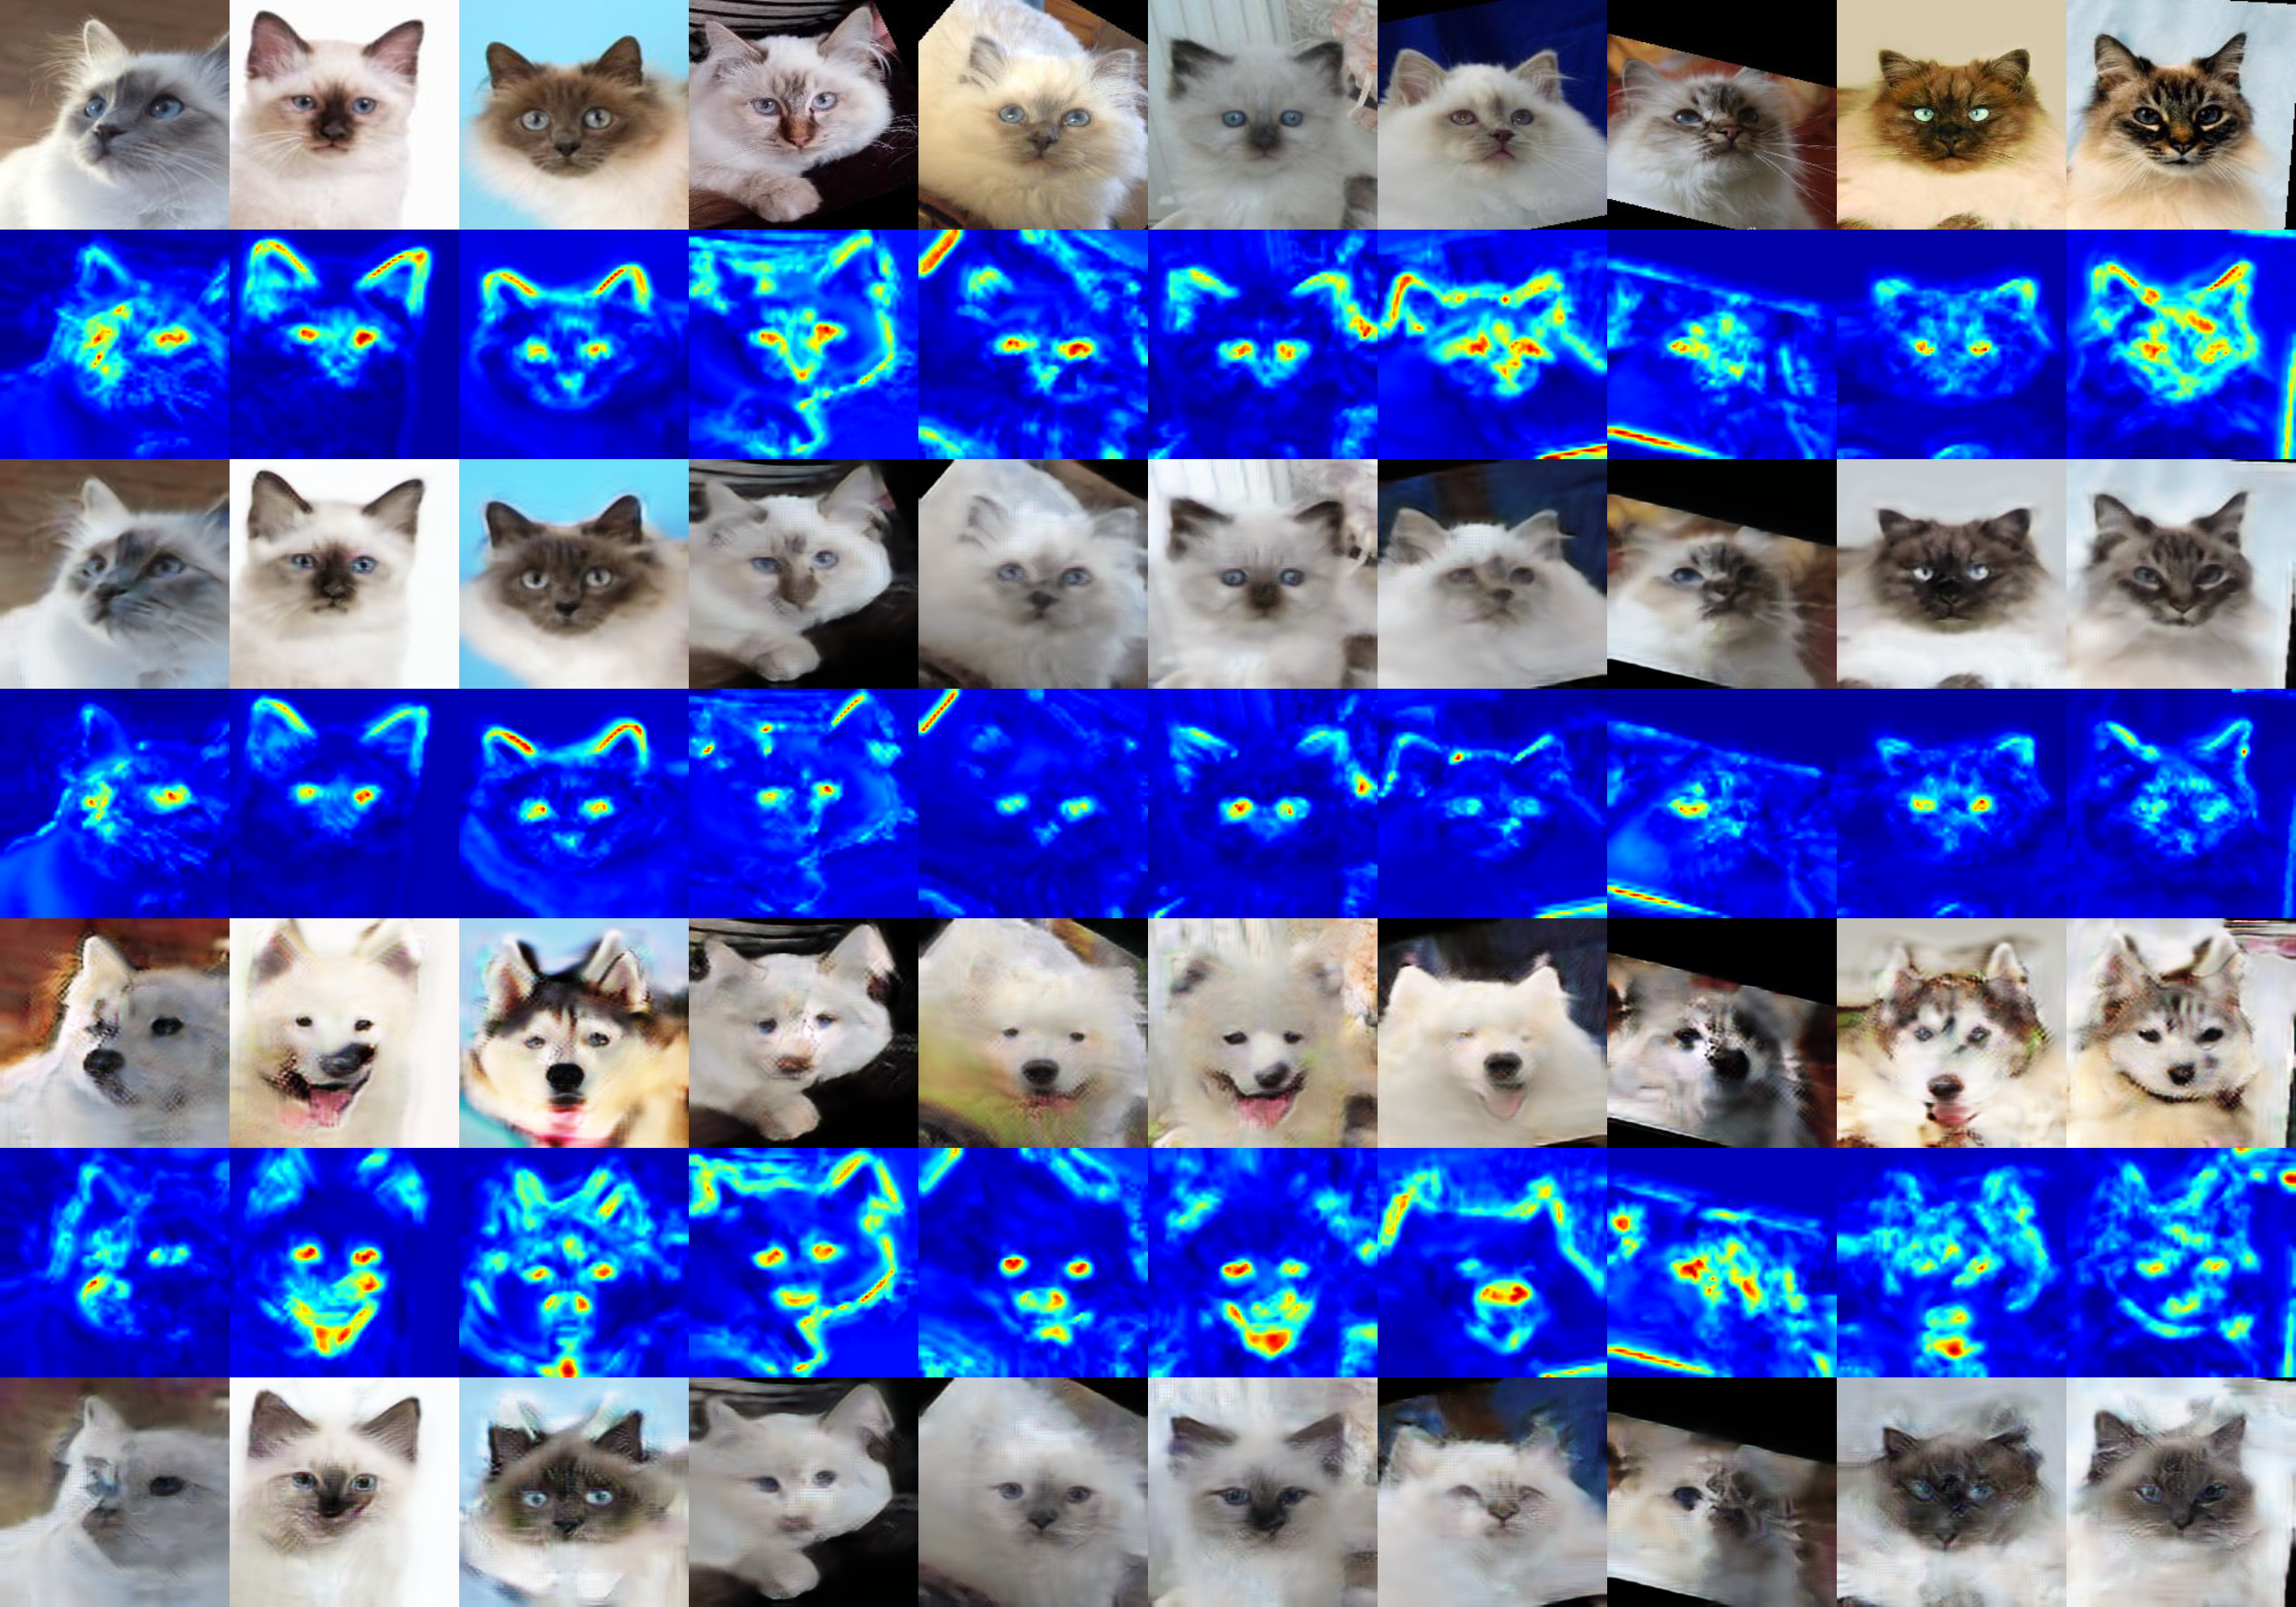
\includegraphics[width=1\columnwidth]{Images/A2B_0020000.png}}\caption{Generated image with heat map on \textbf{cat2dog} dataset after 200 epoch}
\label{fig:cat2dog}
\end{figure} 
By looking at the generated results, we could conclude that our model successfully fulfilled cat to dog translation task despite there are some translated dog images that are not perfect and have some flows. We got very good results on identity mapping since the first row(real\_ A) is almost the same as the third row(idt\_A), which is generated using generator B to A with input A. The fifth row is fake\_B. In a few samples the translation is good and it is difficult to tell whether the image is a real dog or not. However on some other samples especially when the features of cat such as ears or mouth are not obvious, the translated results are not satisfactory. Noticing that the heat map of the eighth sample has more weigh concentrating on the cat's face and there is no clear boundary between features such as ears and mouth. The same thing happened on the last sample, which we can't identify a clear face of dog on fake\_B. The heat map of that sample is unclear and confused, whereas that of other samples has clear bound which depicts the feature of cat. We suppose that it is because of the features of the original image. Depending on the fur color and head position of cats, and image background, there are some features which are hard to be identified through the attention modular. When involving geometrical changes in translating images, a clear boundary between each feature is needed in order to identify each part and translate them into corresponding one.

In order to show the performance improvements of our modified model, we compared the results of our model with the those of CycleGAN model showed in figure\ref{fig:cat2dog}. Each model is trained over 200 epoch. The samples in first row are generated by our modified model and the second row are by original CycleGAN model. For the results of original model, it’s not hard to notice that there is hardly no difference between real\_A and fake\_B, and hence it failed to translate from cat to dog even after 200 epoch. By analyzing the loss of original CycleGAN model, we found that it learned some patterns to reduce the overall loss, yet it didn't understand its task to translating the graphical features of the images.

\begin{figure}
\centerline{\includegraphics[width=1\columnwidth]{Images/compare.png}}\caption{\textbf{cat2dog} results comparison of new model(upper) and CycleGAN(bottom)}
\label{fig:cat2dog}
\end{figure} 

Besides the experiment on \textbf{cat2dog} dataset,  we also ran several experiments on other dataset because we want to ensure that our modified model can not only fulfill image to image translating tasks involving graphical changes but also have good performance on tasks involving texture or color transformation, such as converting horses to zebras. We have prior knowledge that the CycleGAN model is good at texture and color transformation. To justify our thoughts, we also use the CycleGAN model running on the same dataset for comparison. 

\subsubsection{Dataset: \textbf{horse2zebra}}

Figure\ref{fig:horse2zebra} shows the generated image with heat map on \textbf{horse2zebra} dataset after 200 epoch. From this figure we could find out that the horses were indeed converted into zebras and the results are quite satisfactory. In most images the heat map emphasized the shapes of horses, focusing on changing that specific area into texture of zebras. However, there are still some limitations on this model. For example, in the seventh sample where there is a tree beside the horse, even though the weights are concentrated on the horse, the tree is also converted into texture of zebra. Such limitation also happens on CycleGAN according to our experiment results. 


\begin{figure}
\centerline{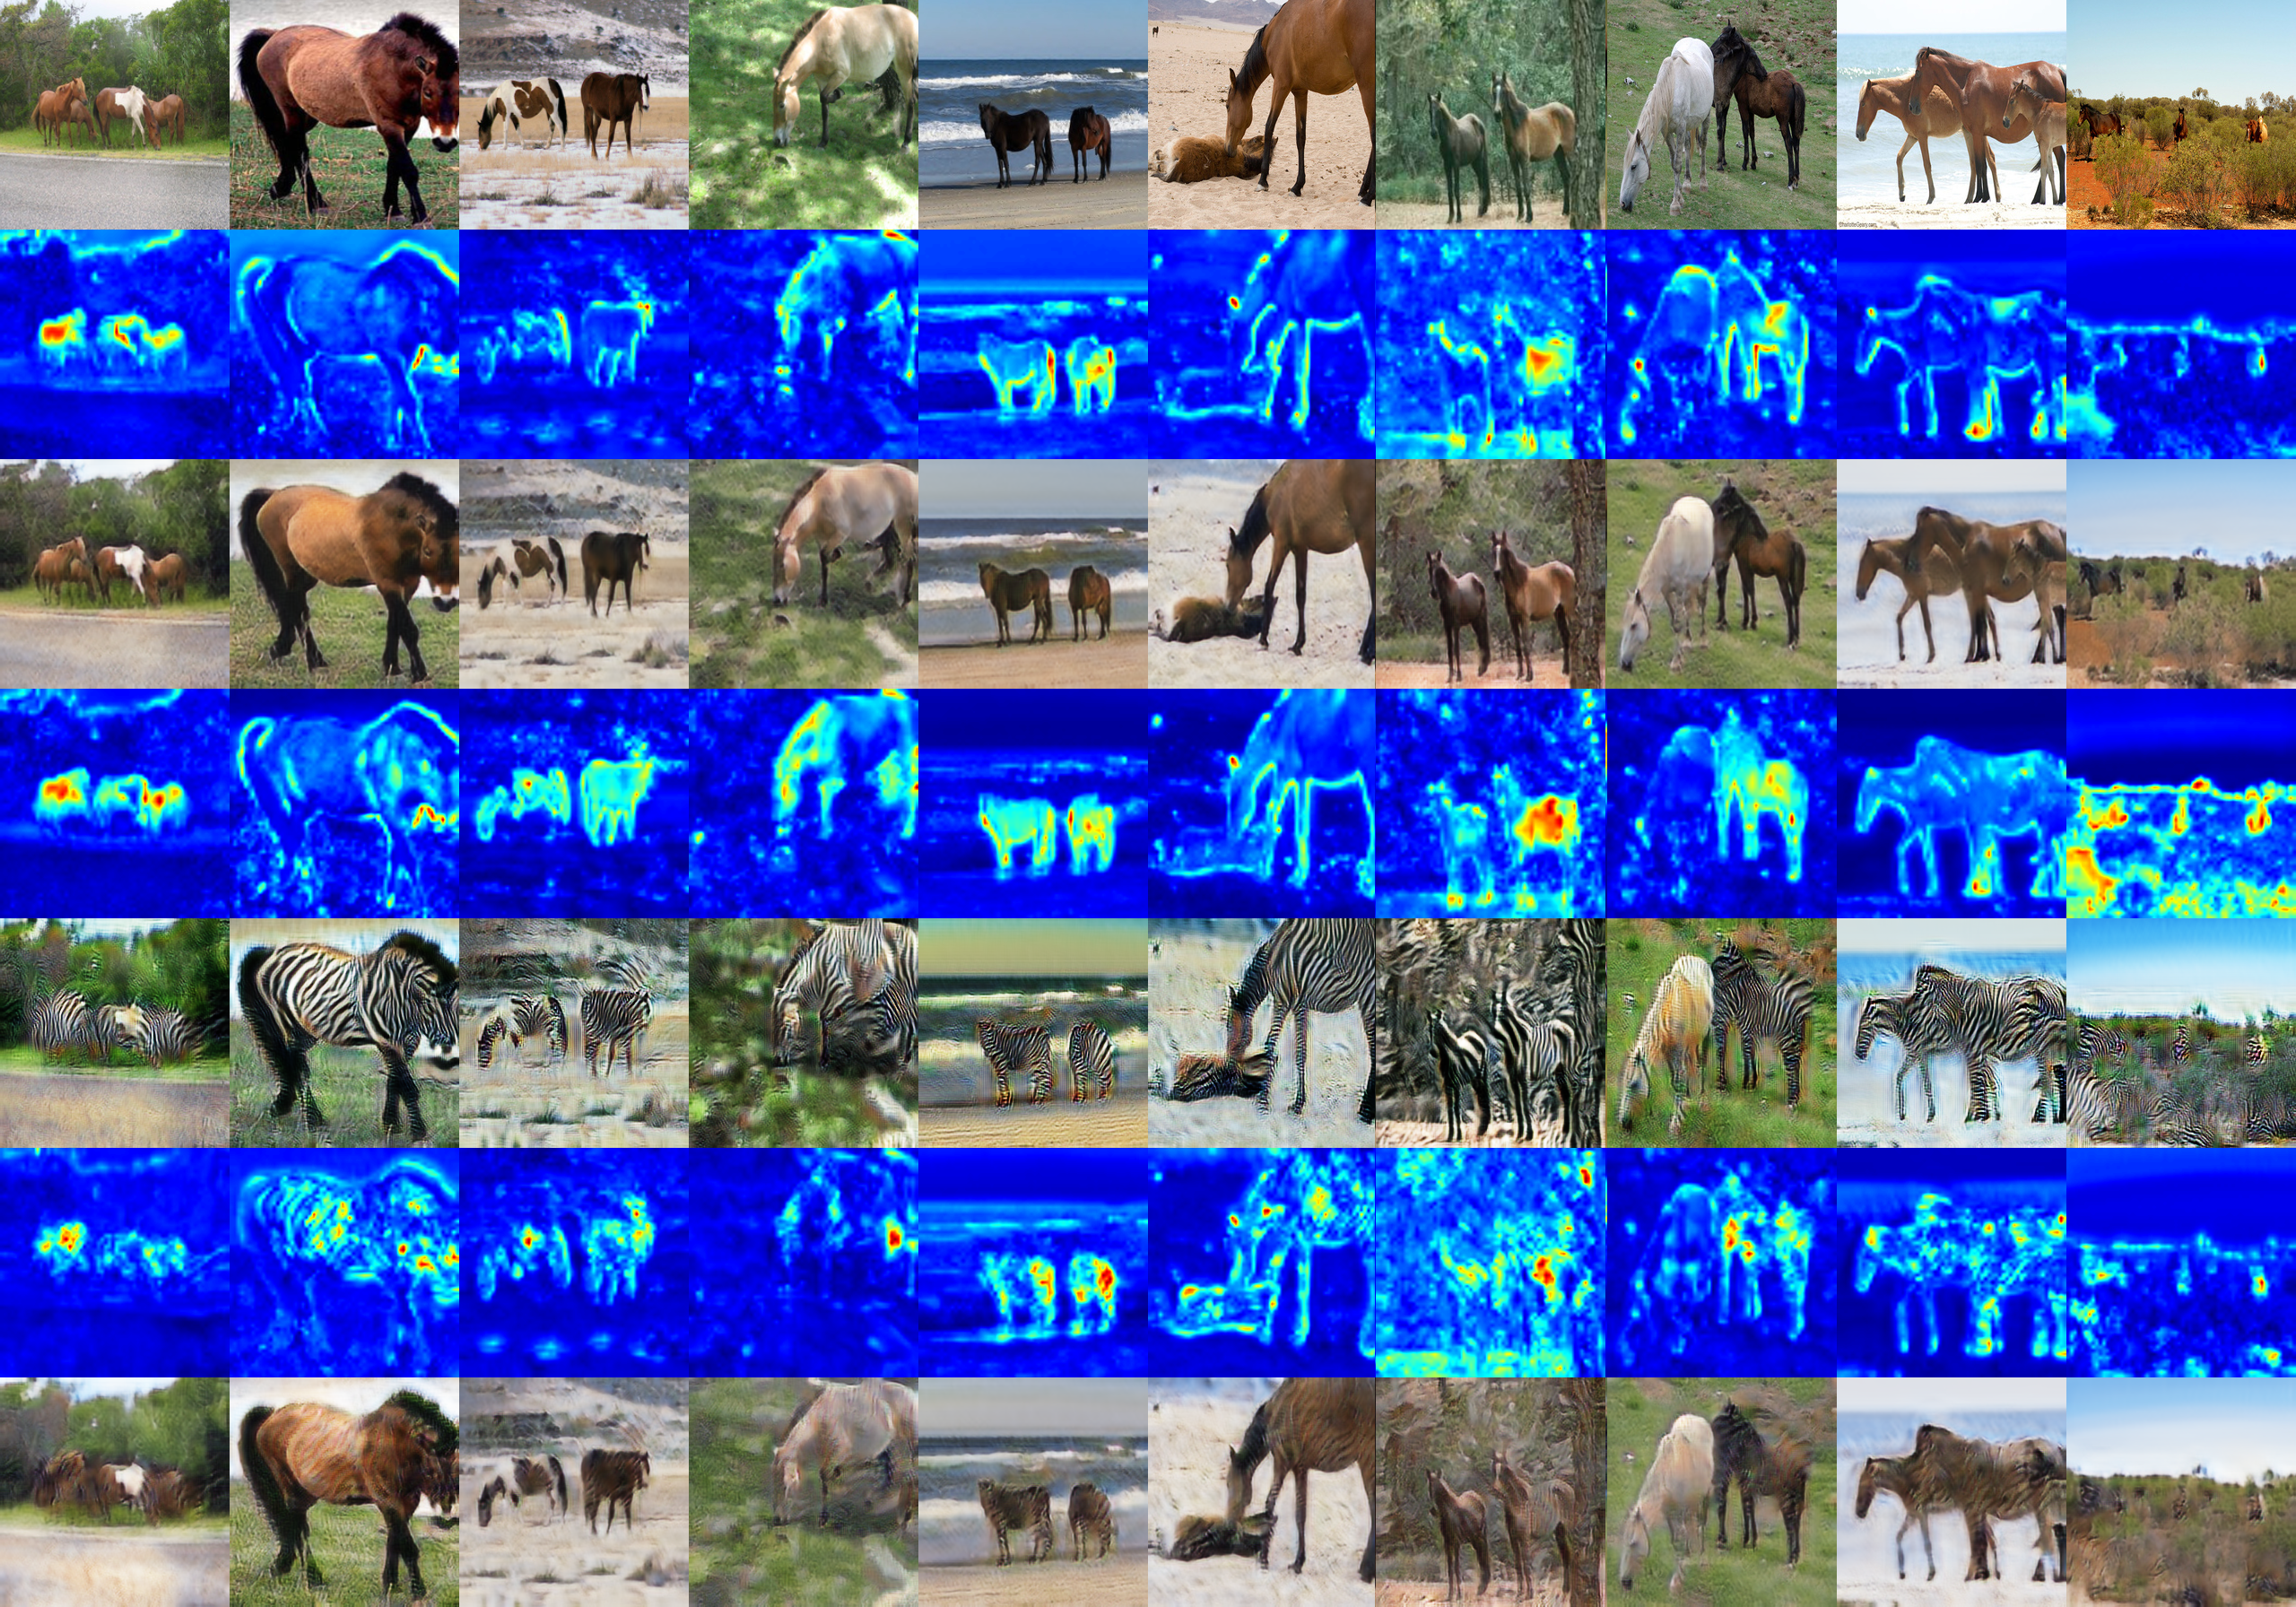
\includegraphics[width=1\columnwidth]{Images/horse2zebra.png}}\caption{Generated image with heat map on \textbf{horse2zebra} dataset after 200 epoch}
\label{fig:horse2zebra}
\end{figure} 

Figure\ref{fig:horse2zebra_compare} is the comparison of generated images for \textbf{horse2zebra} dataset. The upper samples are generated using modified model and the bottom are from CycleGAN model. Generally, there are no much differences between results for both models, except for the color of background or texture, but such nuance won't affect overall performance.

\begin{figure}
\centerline{\includegraphics[width=1\columnwidth]{Images/horse2zebra_compare.png}}\caption{\textbf{horse2zebra} results comparison of new model(upper) and CycleGAN(bottom)}
\label{fig:horse2zebra_compare}
\end{figure} 

\subsubsection{Results for other dataset}

In order to check whether our modified model could outperform the original CycleGAN model on various dataset, we tested them with different dataset. The results for the rest experiments on dataset \textbf{apple2orange}, \textbf{summer2winter} and \textbf{iphone2dslr\_flower} are showed in figure\ref{fig:meta_compare}. In these experiments we found that not all tasks involving color and texture transformation could be solved using the existing model. 

\begin{figure}
\centerline{\includegraphics[width=1\columnwidth]{metacompare.png}}\caption{\textbf{apple2orange}, \textbf{summer2winter}, \textbf{iphone2dslr\_flower} dataset results comparison of new model(upper) and CycleGAN(bottom)}
\label{fig:meta_compare}
\end{figure} 

The first two columns are for experiments on \textbf{apple2orange} dataset. In this task, the biggest problem is that neither our model nor CycleGAN model successfully remove the pedicel of the apple, which is absolutely not on oranges. We suggest that it is because this feature is relatively small that the attention module can't catch up this feature. The images in the middle two columns are for experiments on \textbf{summer2winter} dataset. In our results there is nothing changed between real\_A and fake\_B and hence our modfified model failed to do this task. The last two columns are for experiments on \textbf{iphone2dslr\_flower} dataset. Different from previous experiments, this task aims to enhance the image qualities by improving the quality of photos taken by iPhone to the quality of photos taken by DSLR. Image enhancement is another kind of features for CycleGAN and we want to test that if our modified model could also do this kind of task. According to the results, the image translated by CycleGAN has higher quality and richer colors than ours. In summary, the overall results of these five datasets for both models are showed in table\ref{tab:overall}.

\begin{table}[tb]
\vskip 3mm
\begin{center}
\begin{small}
\begin{sc}
\begin{tabular}{lcccr}
\hline
\abovespace\belowspace
Data set & Better than CycleGAN? \\
\hline
cat2dog    & $\surd$ \\
horse2zebra & $\surd$\\
apple2orange & $\surd$ \\
summer2winter  &   $\times$\\
iphone2dslr\_flower & $\times$ \\

\hline
\end{tabular}
\end{sc}
\end{small}
\caption{Overall performance on different dataset}
\label{tab:overall}
\end{center}
\vskip -3mm
\end{table}

\subsubsection{Special experiment}

We did an extra experiment on dataset \textbf{selfie2anime} due to the special feature of the network architectures which we adapted from UGATIT\cite{U-GAT-IT}. According to their work, the UGATIT model could fulfill image style translation such as converting a realistic photo to anime. The author showed the results of anime-style transfer and the performance was really nice. Hence we ran the \textbf{selfie2anime} dataset on our modified model to check whether we could achieve the same performance as UGATIT. 

\begin{figure}[H] 
    \centering
    \subfloat[Real A]{%
        \quad\includegraphics[height=1in]{Images/selfie.png}\quad%
        }%
    \hspace*{.4in}
    \subfloat[Fake B]{%
    \quad\includegraphics[height=1in]{Images/anime.png}\quad%
        }%
    \caption{\textbf{selfie2anime} dataset results}
    \label{fig:selfie2anime}
\end{figure}

Figure\ref{fig:selfie2anime} shows the results of \textbf{selfie2anime} dataset. The overall style is anime though, there are some confused part in the generated image, such as the ambiguous boundary between hair and close, big and small eyes, and meaningless background. This outcome is below our expectation. We suggest that it might be due to the dataset we used in this experiment. We found that the distribution of selfie and anime are quite different. For example, in training examples of selfie, people wear glasses, use cellphone, make different poses, all of which have no corresponding items in anime. On the other hand, there are some characteristics in anime samples such as exaggerated head to body ratio which doesn't exist in realistic. Such discrepancy made it hard to do the selfie to anime translation, and we would only get good results on limited samples.



\if
This section should cover the experiments carried out, including, for each experiment, the:
\begin{itemize}
    \item  Motivation -- what did you aim to learn from the experiment?
    \item  Baselines -- do you compare your method to appropriate baselines (e.g. the existing method that you built on your method)?
    \item  Description -- describe carefully how you carried out the experiment, mentioning and justifying the hyperparameter settings. As always, your aim is to give enough information so that someone else (e.g. another MLP group) could reproduce the experiment precisely.
    \item  Results -- present the results clearly and concisely. Usually a result is in comparison to a result from another approach (e.g. a baseline experiment, the previous experiment, results from the literature, \dots).  Please make sure that these comparisons are clearly presented.
    \item Interpretation and discussion -- what do your results indicate? how do they relate to the motivation for the experiment? are there further useful analyses or visualisations of the results that you can carry out?
\end{itemize}

Please note that negative results are not necessarily a bad thing -- learning is always good! But negative or positive, please try to analyse your results as well as you can.

There is no need to include code or specific details about the compute environment.

As before, your experimental sections should include graphs (for instance, figure~\ref{fig:sample-graph}) and/or tables (for instance, table~\ref{tab:sample-table})\footnote{These examples were taken from the ICML template paper.}, using the \verb+figure+ and \verb+table+ environments, in which you use \verb+\includegraphics+ to include an image (pdf, png, or jpg formats).  Please export graphs as 
\href{https://en.wikipedia.org/wiki/Vector_graphics}{vector graphics}
rather than \href{https://en.wikipedia.org/wiki/Raster_graphics}{raster
files} as this will make sure all detail in the plot is visible.
Matplotlib supports saving high quality figures in a wide range of
common image formats using the
\href{http://matplotlib.org/api/pyplot_api.html\#matplotlib.pyplot.savefig}{\texttt{savefig}}
function. \textbf{You should use \texttt{savefig} rather than copying
the screen-resolution raster images outputted in the notebook.} An
example of using \texttt{savefig} to save a figure as a PDF file (which
can be included as graphics in a \LaTeX document is given in the coursework document.

If you need a figure or table to stretch across two columns use the \verb+figure*+ or \verb+table*+ environment instead of the \verb+figure+ or \verb+table+ environment.  Use the \verb+subfigure+ environment if you want to include multiple graphics in a single figure.

\begin{figure}[tb]
\vskip 5mm
\begin{center}
\centerline{\includegraphics[width=\columnwidth]{icml_numpapers}}
\caption{Historical locations and number of accepted papers for International
  Machine Learning Conferences (ICML 1993 -- ICML 2008) and
  International Workshops on Machine Learning (ML 1988 -- ML
  1992). At the time this figure was produced, the number of
  accepted papers for ICML 2008 was unknown and instead estimated.}
\label{fig:sample-graph}
\end{center}
\vskip -5mm
\end{figure} 

\begin{table}[tb]
\vskip 3mm
\begin{center}
\begin{small}
\begin{sc}
\begin{tabular}{lcccr}
\hline
\abovespace\belowspace
Data set & Naive & Flexible & Better? \\
\hline
\abovespace
Breast    & 95.9$\pm$ 0.2& 96.7$\pm$ 0.2& $\surd$ \\
Cleveland & 83.3$\pm$ 0.6& 80.0$\pm$ 0.6& $\times$\\
Glass2    & 61.9$\pm$ 1.4& 83.8$\pm$ 0.7& $\surd$ \\
Credit    & 74.8$\pm$ 0.5& 78.3$\pm$ 0.6&         \\
Horse     & 73.3$\pm$ 0.9& 69.7$\pm$ 1.0& $\times$\\
Meta      & 67.1$\pm$ 0.6& 76.5$\pm$ 0.5& $\surd$ \\
Pima      & 75.1$\pm$ 0.6& 73.9$\pm$ 0.5&         \\
\belowspace
Vehicle   & 44.9$\pm$ 0.6& 61.5$\pm$ 0.4& $\surd$ \\
\hline
\end{tabular}
\end{sc}
\end{small}
\caption{Classification accuracies for naive Bayes and flexible 
Bayes on various data sets.}
\label{tab:sample-table}
\end{center}
\vskip -3mm
\end{table}

\fi


\section{Related work}
\label{sec:relwork}
\subsection{Generative Adversarial Networks (GANs)}
Generative Adversarial Networks (GANs) \cite{GAN} have demonstrated remarkable performance in image generation \cite{image_generation_1}\cite{image_generation_2}\cite{image_generation_3}, image editing \cite{image_editing}, image inpainting \cite{image_inpainting}, image translation \cite{image_translation_1}\cite{image_translation_2}, and representation learning \cite{representation_learning}. The generator attempts to produce realistic pictures in order to deceive the discriminator, while the discriminator attempts to separate the generated image from the real image, which is made possible by GAN's concept of adversarial loss. The concept has recently gained widespread use in applications such as conditional picture creation \cite{text2image} and other domains such as 3D data \cite{3D}. The emergence of GANs permits translation from a source domain to a radically different destination domain provided unpaired training data \cite{Conditional_GANs}.

\subsection{Image-to-Image Translation}
The concept of image-to-image translation can be traced back to Image Analogies \cite{Image_Analogies}, in which Hertzmann used a single input-output training image pair to train a nonparametric texture model. Isola presented a unified framework for image-to-image translation based on conditional GANs, dubbed "pix2pix" \cite{Conditional}. The "pix2pix" framework employs conditional generative adversarial networks to learn the mapping between the input and output images \cite{AL}. CycleGAN's approach also makes use of this framework \cite{Cycle}, since it is used to learn parametric translation from a dataset of input and output instances \cite{CNN}. These concepts have been applied to a variety of techniques, including image generation from sketches \cite{Scribbler} or semantic layouts \cite{Semantic_Layouts}. Recently, a high-resolution version of the "pix2pix" framework was developed \cite{Conditional_GANs}. UNIT provides a shared workspace for unsupervised image translation \cite{UNIT}. MUNIT decomposes images into domain-invariant content codes and domain-specific style codes \cite{image_translation_2}. DRIT decomposes images into their constituent content and styles \cite{DIRT}, enabling MUNIT to do many-to-many mapping. AGGAN enhances image translation performance by utilising an attention mechanism to discern foreground from background \cite{AGGAN}. Although the idea of attention is novel and the experiment has a forward-looking directing impact, the indicator does not improve significantly.

\subsection{Cycle Consistency}
The concept of cycle consistency has gained more and more attention in data structure. Translators \cite{translators} and translation machines \cite{translation_machines} are rapidly embracing technological advances in their job of language translation, namely reverse translation and altering matching logic to test the correctness of translation, which may be improved by repeated verification. Visual tracking is constantly emphasising the consistency of attributes prior to and following the change \cite{visual_tracking}. Cyclic consistency is being developed at a breakneck pace and has already produced remarkable achievements in the following areas: structural analysis under grasping motion state \cite{motion_state}, high-precision 3D model matching \cite{3D_Model}, adaptive dense semantic communities \cite{dense_semantic}, and deep-level estimation \cite{deep-level}. It is worthwhile to learn a translation approach inspired by machine translation that can employ a similar purpose of capturing the invisible traits of unpaired images \cite{DualGAN}.

\subsection{Class Activation Map (CAM)}
Class Activation Map (CAM) was proposed through utilising global average pooling in a CNN \cite{Discriminative}. The CNN uses the CAM for a certain class to identify the image patches that may be used to make a distinction.

\subsection{Normalization}
Recent studies on neuronal style transfer have demonstrated that CNN feature statistics may be employed directly as descriptors of visual styles \cite{Gram_matrix}. By normalising the image's extracted features, Instance Normalization (IN) eliminates stylistic variance. Recent researches, however, have discovered that when normalising images, Conditional Instance Normalization (CIN) \cite{CIN} and Batch-Instance Normalization (BIN) \cite{Batch-Instance} are superior to IN alone.

\section{Conclusions}
\label{sec:concl}

In summary, the overall performance of our model is consistent with our expectations based on the results of those six experiments, though it still has many flaws and defects. In cat to dog transferring task, the model shows its ability to make geometrical translations in images. The attention module helps the model focus more on the features of source domain and target domain which made the geometrical change more precise. On texture and color transferring tasks, the model is also competent to carry out this kind of work, despite that the performance is not as good as CycleGAN on some certain dataset. It can be inferred that a model which performs good on tasks with geometrical changes doesn't represent that it can also perform good on tasks with texture and color changes. Additionally, we also tried to reproduce the results of selfie to anime tasks which is mentioned in the paper of UGATIT\cite{U-GAT-IT}. However, we found it difficult to achieve the same performance as the authors did.


While our method produces acceptable outcomes in the great majority of circumstances, certain results are inconsistently satisfactory. In terms of contour judgement, our method cannot be completely accurate in identifying the attribution of contours with dominant chromatic aberration or invisible traits, since this is dependent on the threshold configuration of the discriminator for contour judgement. This is more dominantly reflected in the process of converting a horse into a zebra, which can be accomplished entirely even while the horse is partially concealed. The issue is that in such a case, if a person performs a similar movement, our method is likely to misidentify it and converted into a zebra man. To solve this issue, further effort may need optimising the discriminator's attention in order to properly locate object outlines by the incorporation of additional external features.

Another noticeable flaw is that it is difficult for the generator to convert the original data set with obvious morphological changes to the target data set in order to accomplish an entirely perfect conversion, which can also serve as a direction for future research. The generator is not capable of concealing or erasing morphological traits that should not be present in the generated target yet are. A more typical case occurs when apples are converted to oranges, as apples include pedicels in their natural state, which oranges normally lack, yet our method makes it impossible to obscure or eliminate this trait.

\if
The conclusions section should concisely summarise what you have learned from the experiments you carried out, and relate the final outcome of the project to the overall research questions and objectives. If there were potentially interesting future directions in your project that you could not explore due to lack of time and/or space, mention them briefly.
\fi



\bibliography{example-refs}

\end{document} 

